\documentclass[10pt,conference]{IEEEtran}
\IEEEoverridecommandlockouts
% The preceding line is only needed to identify funding in the first footnote. If that is unneeded, please comment it out.
\usepackage{cite}
\usepackage{amsmath,amssymb,amsfonts}
\usepackage{algorithmic}
\usepackage{graphicx}
\graphicspath{{figures/}}
\usepackage[spaces,hyphens]{xurl}
\usepackage{textcomp}
\usepackage{xcolor}
\def\BibTeX{{\rm B\kern-.05em{\sc i\kern-.025em b}\kern-.08em
    T\kern-.1667em\lower.7ex\hbox{E}\kern-.125emX}}

\begin{document}

\title{An Exploratory Study of Project Activity Changepoints in Open Source Software Evolution}

\author{\IEEEauthorblockN{James Walden}
\IEEEauthorblockA{\textit{Department of Computer Science} \\
\textit{Northern Kentucky University}\\
Highland Heights, KY USA\\
waldenj@nku.edu}
\and
\IEEEauthorblockN{Noah Burgin}
% \IEEEauthorblockA{\textit{Department of Electrical Engineering\\ and Computer Science} \\
 \IEEEauthorblockA{\textit{Department of EE and Computer Science} \\
    \textit{University of Tennessee}\\
Knoxville, TN USA\\
noah22@vols.utk.edu}
\and
\IEEEauthorblockN{Kuljit Kaur}
\IEEEauthorblockA{\textit{Department of Computer Science} \\
\textit{Guru Nanak Dev University}\\ 
Amritsar, India\\
kuljitchahal.cse@gndu.ac.in} 
}
\maketitle

\begin{abstract}
We applied changepoint analysis methods to a dataset of open source projects in order to determine the smoothness of open source evolution.
We used a nonparametric changepoint detection algorithm on a dataset of 8,919 projects with at least four years of project activity selected from the World of Code, searching for changepoints in the number of commits and the number of unique contributing authors per month.
We show that 99\% of projects have changepoints in both time series, with a typical range between one and six changepoints. Increases and decreases in project activity occur with about equal frequency, while the size of changes varies tremendously.
\end{abstract}

\begin{IEEEkeywords}
software evolution, changepoints
\end{IEEEkeywords}

\section{Introduction}

We performed an exploratory study of changepoints in open source project activity during the MSR 2021 hackathon. We analyzed project activity time series obtained from the World of Code~\cite{ma2019world}, an archive cross-referencing over 120 million git repositories from multiple forges. We selected 8,919 projects from the World of Code that had sufficient history to compute monthly time series of commit activity, author activity, and the number of files changed.

Changepoints are data points in a time series, where the statistical properties of the data points before and after the changepoint differ significantly. While Lehman's laws of software evolution~\cite{lehman1996laws} point towards general tendencies of software evolution, such as increasing number of features and complexity, these laws do not describe whether a project gradually follows those trends or whether a project moves slowly at one point then rapidly at another point in its evolution.

Changepoint analysis has previously been used to identify instances when software performance changed~\cite{cito2014identifying,muhlbauer2020identifying}. Two prior case studies of open source projects visually identified changepoints in development activity of a single project~\cite{gonzalez2014studying,openssl2020} without using a changepoint detection algorithm. 

We focused our study on two research questions:
\begin{enumerate}
    \item How common are changepoints in open source project activity?
    \item What are the sizes and directions of changes at changepoints?
\end{enumerate}

\section{Data}

We selected projects from the World of Code~\cite{ma2019world}, a research archive containing billions of commits from free, libre, and open source software (FLOSS) git repositories. In order to have a sufficiently long time series for changepoint analysis, we chose projects that had at a lifespan of at least four years, with at least 50 authors and 5000 commits. We found 8,919 projects that met our criteria.

We identified projects that met our criteria using the MongoDB \texttt{WoC.proj\_metadata.R}. During the course of the multiweek virtual hackathon, World of Code transitioned from version R to S. We adapted our data collection scripts and procedures to use the new version S, in order to gain access to the new \texttt{rootfork} field it provided. Forges like GitHub contain many forks of popular projects, making it difficult to identify the repository that is used by the project team for development. Prior to version S, the only measure of centrality in a cluster of projects was algorithmically determined within WoC. The \texttt{rootfork} field was retrieved from GitHub, and therefore is the true root project.

We collected three monthly time series for each project: number of commits, number of unique authors, and number of files changed per commit. Time series were computed using the \texttt{getValues} commands that access data in pre-computed maps and tables within WoC. To get all commits for a certain project, we used the \texttt{p2c} map. These commits were then piped to \texttt{c2ta} to retrieve the timestamp and author of each commit. From here, a python script grouped each commit by month and counted the number of commits per month and how many unique authors made those commits in that month.

\textbf{Noah:} Can you provide performance data for both project selection and computing time series?

Since World of Code does not provide a map from commits to time and files changed, we used WoC's python interface, \texttt{oscar.py} to compute time series for the number of files changed. Commit objects in the python interface provided the needed timestamps and files changed per commit data. Commits were grouped by month and were used to compute the number of files changed per month.

\textbf{Noah:} Can you explain the zero size and zero row time series files I found? What about the post-2020 dates?\\

\section{Changepoint analysis}

As our time series data was not normally distributed, we used a nonparametric algorithm to detect changepoints. In particular, we used the implementation of the nonparametric PELT algorithm found in version 1.0.2 of the R \texttt{changepoint.np} package~\cite{killick2014changepoint}. We used the algorithms default parameters, with the exception of specifying the minimum segment length be three months, as we wanted to find changes in activity that were at least slightly durable instead of looking for anomalous months. 

We did not perform hyperparameter optimization, as we did not have a dataset of project activity time series with labeled changepoints to evaluate algorithm performance. An evaluation of multiple changepoint algorithms on a variety of time series~\cite{van2020evaluation} from different fields of study found little improvement from hyperparameter optimization of this algorithm in any case.

We found that more than 99\% of projects have changepoints in project activity. Only 55 projects had no changepoints in their author time series, with most projects having between one and five changepoints. There are outliers, with six projects having 10 changepoints and one project having 14 changepoints. No project had between 11 and 13 changepoints. We can see the distribution of projects by number of changepoints in Figure~\ref{fig:authorcpts}.
\begin{figure}[ht!]
    \centering
    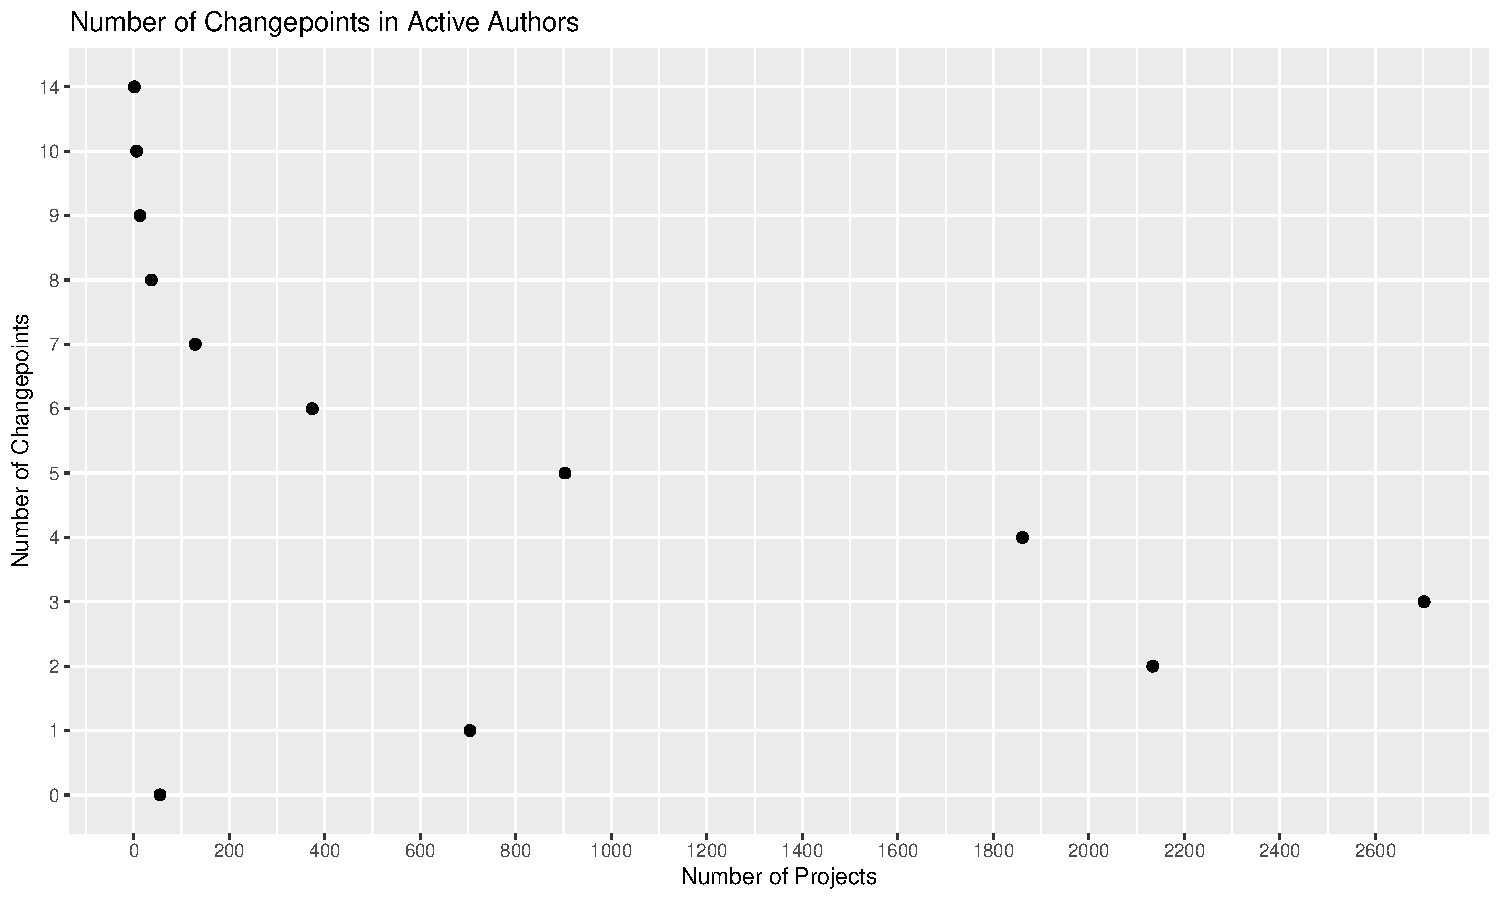
\includegraphics[width=\linewidth]{author-changepoints.pdf}
    \caption{Number of Changepoints in Author Time Series}
    \label{fig:authorcpts}
\end{figure}

Only 32 projects had no changepoints in their commit time series, with most projects having between one and six changepoints. Outliers include 27 projects with ten or more changepoints, with a single project having 16 changepoints.
\begin{figure}[ht!]
    \centering
    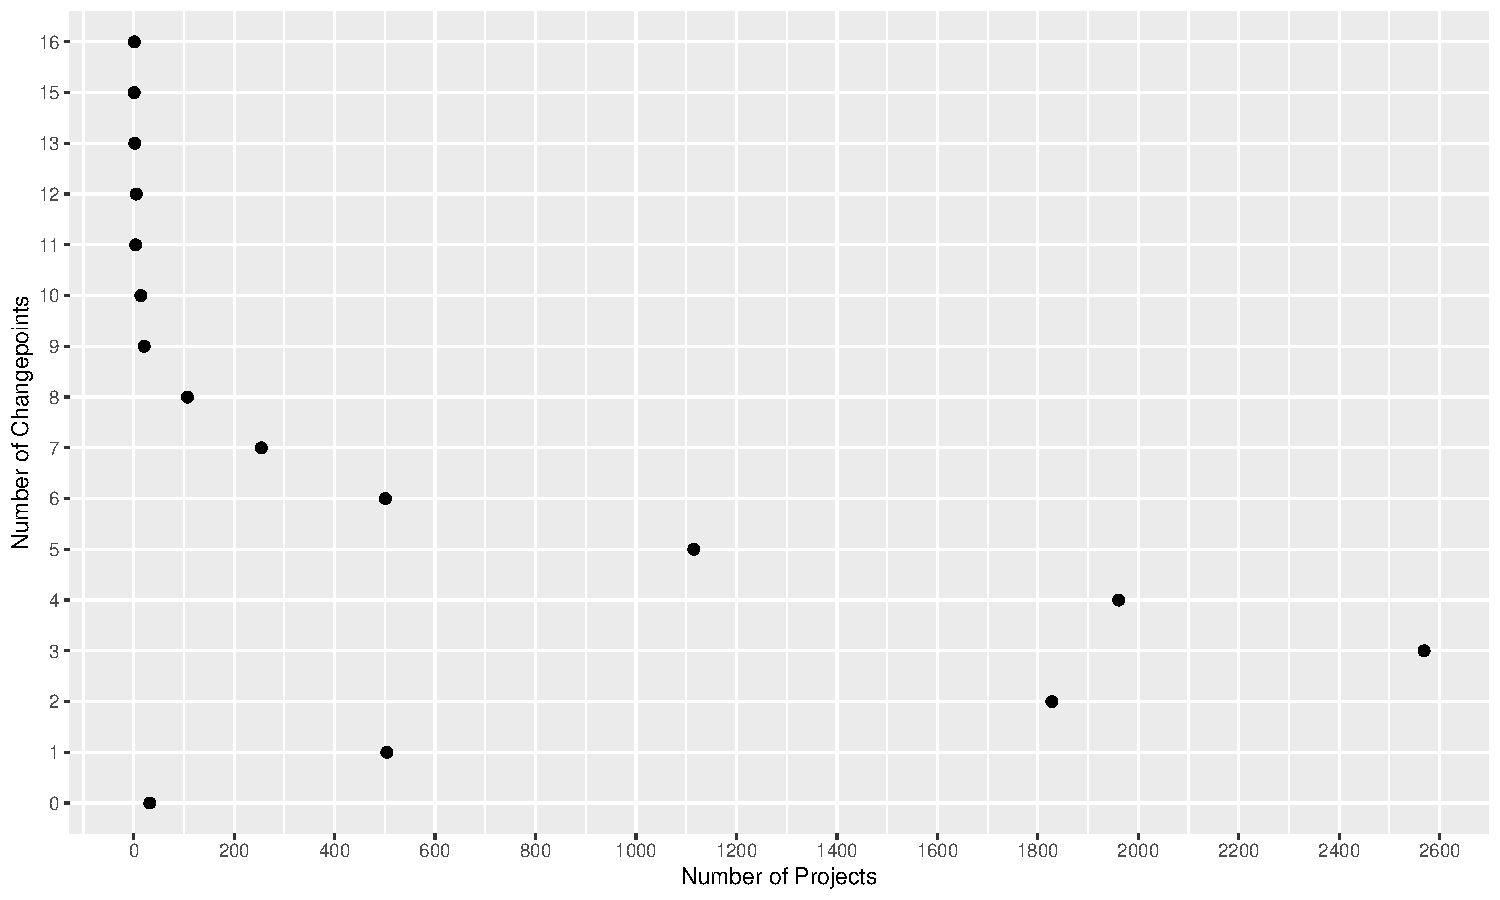
\includegraphics[width=\linewidth]{commit-changepoints.pdf}
    \caption{Number of Changepoints in Commit Time Series}
    \label{fig:commitcpts}
\end{figure}

We found a total of 31,416 changepoints in project commit time series, of which 15,342 (48.8\%) were increases in commit activity and 16,047 (51.1\%) were reductions in activity. We computed the magnitude of a changepoint as the difference in means in the number of monthly commits before and after the changepoint. The size of most changes were relatively small, with the interquartile range (IQR) ranging between -75 to 87 commits per month, but there was a substantial tail in both directions as can be seen in Figure~\ref{fig:commitsizes}.
\begin{figure}[ht!]
    \centering
    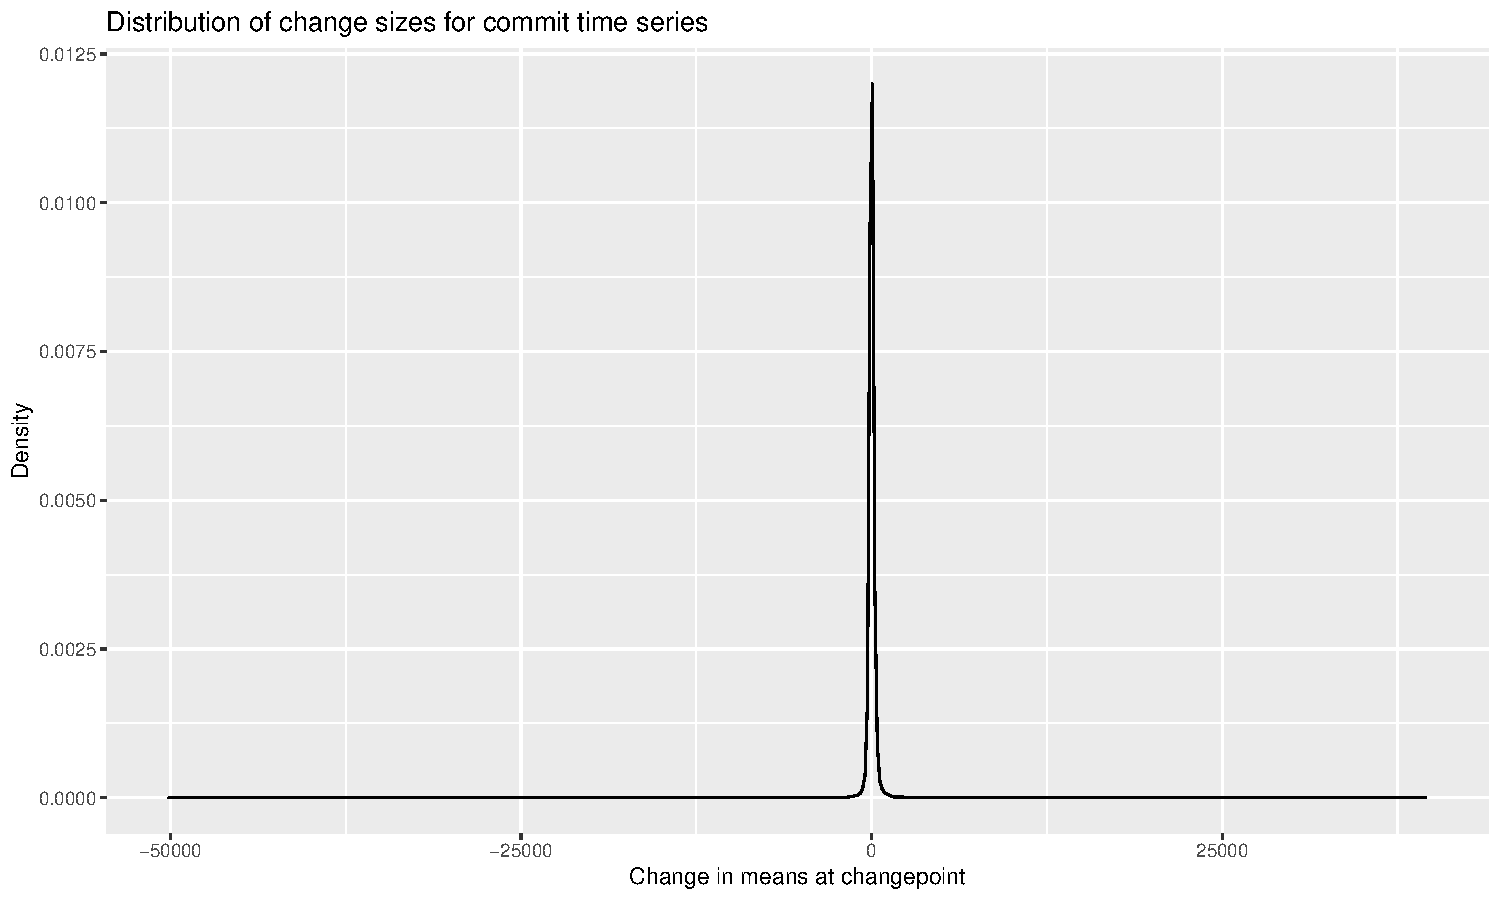
\includegraphics[width=\linewidth]{commit-changesizes.pdf}
    \caption{Size of Changes in Commit Time Series}
    \label{fig:commitsizes}
\end{figure}

Our results for the signs and magnitude of author time series changes were similar. We found 28,671 changepoints in author time series, of which 12,114 (42.2\%) were reductions in activity and 16,557 (57.7\%) were increases in activity. Changes in the number of contributing authors per month were relatively small, with IQR ranging between -3.4 to 5.8 authors per month, but there was a substantial tail in both directions as can be seen in Figure~\ref{fig:authorsizes}.
\begin{figure}[ht!]
    \centering
    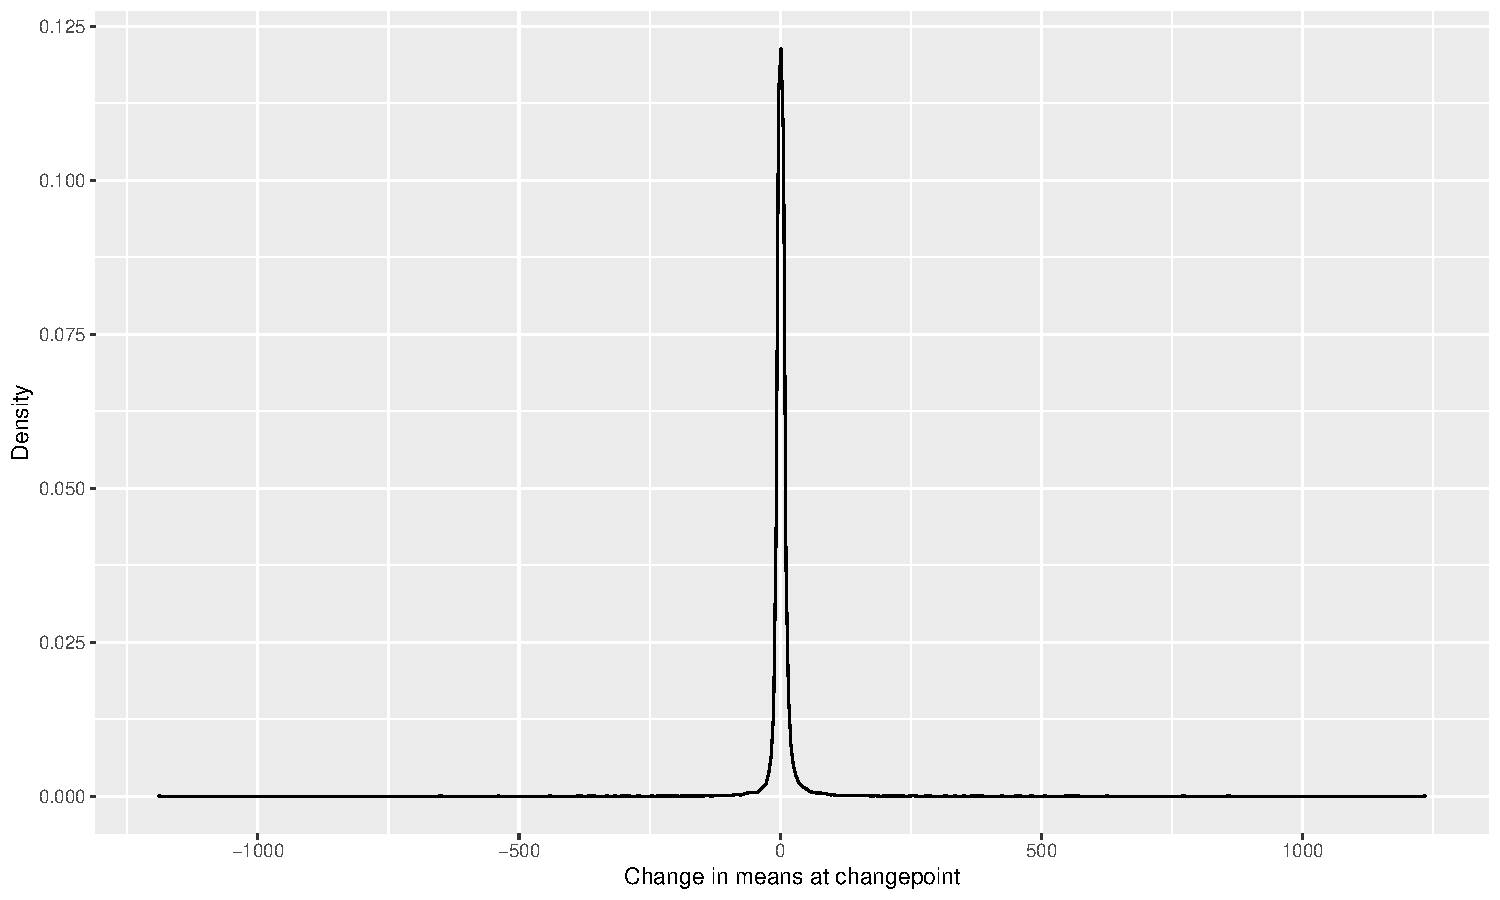
\includegraphics[width=\linewidth]{author-changesizes.pdf}
    \caption{Size of Changes in Author Time Series}
    \label{fig:commitsizes}
\end{figure}


\section{Conclusion}

We found that open source evolution is rarely smooth and typically includes changepoints, points where the size and/or direction of evolution changes significantly. 

The data and code used in this project can be found in the project's git repository at \url{https://github.com/woc-hack/inflection-points}.

In the future, we would like to examine our data in more detail to identify if there are common patterns of changepoints in open source evolution and to see what makes the outliers in number and magnitude of changepoints so different from the majority of projects. We would also like to gather WoC \texttt{P2c} commit time series data, which provides commits for all projects in a cluster. This would allow us to understand how the community’s contributions to a project evolve rather than inspecting a single project at a time.


\bibliographystyle{IEEEtran}
\bibliography{changepoints-msr2021}

\end{document}
